\documentclass{article}
\usepackage{graphicx}
\usepackage[]{mdframed}
\usepackage{tabularx}
\usepackage{subfig}
\usepackage{placeins}
\usepackage{float}
\usepackage{parskip}

\graphicspath{ {./graphing/} }
\usepackage[a4paper, total={6in, 8in}]{geometry}

\newcolumntype{Y}{>{\centering\arraybackslash}X}

\author{Sidharth Babu, SNB2593 \and Tianda Huang, TH32684}
\title{ECE 361E: Homework 3}

\begin{document}
\begin{mdframed}
    \maketitle
\end{mdframed}
\pagebreak

\section*{Problem 1}
\subsection*{Question 2}
\begin{figure}[!htb]
    \caption{\textit{Table 1}}
    \begin{tabularx}{\textwidth}{|*{7}{Y|}}
        \hline
        Model & Training Accuracy [\%] & Test Accuracy [\%] & Total Time for Training [s] & Number of Trainable Params & Floating Point Operations & GPU Memory, Training (MiB)\\
        \hline
        VGG11 & 97.57 & 76.48 & 3011.79 & 9,750,922 & 306,587,648 & 2583 \\
        \hline
        VGG16 & 97.86 & 78.89 & 3622.42 & 14,655,050 & 551,954,432 & 2583 \\
        \hline
        MobileNet & 99.42 & 77.75 & 2211.56 & 3,217,226 & 96,002,048 & 1151\\
        \hline
    \end{tabularx}
    \label{fig:model-summary}
\end{figure}

\subsection*{Question 3}
\begin{figure}[!htb]
    \centering
    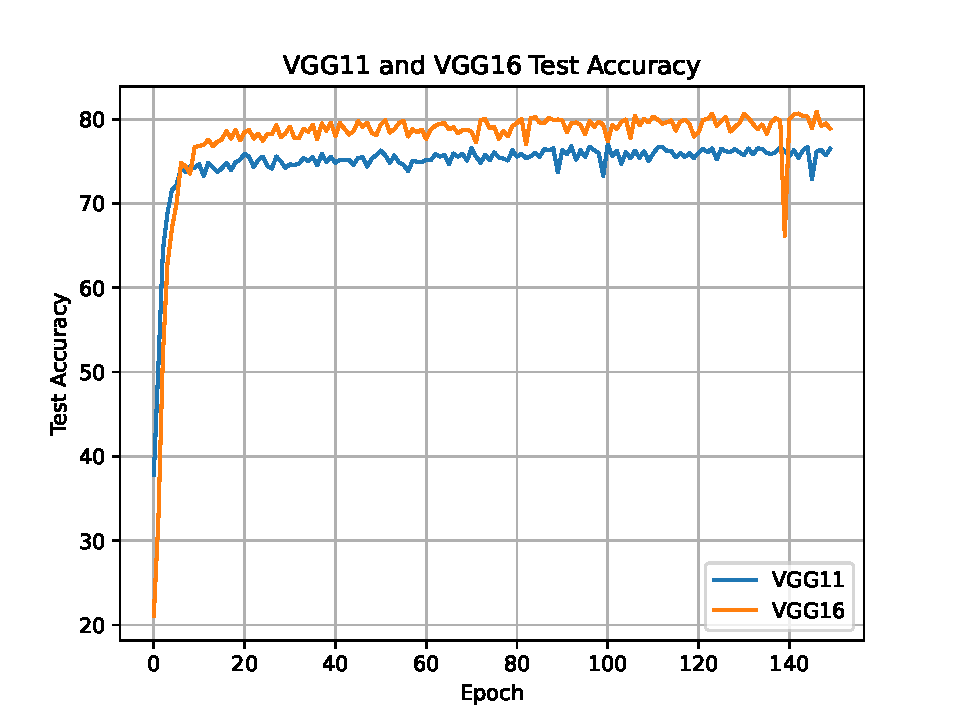
\includegraphics[width=\textwidth]{vgg11_16_acc.pdf}
    \caption{Test Accuracy of VGG11 and VGG16}
    \label{fig:vgg-epoch-accuracy}
\end{figure}

There exists a tradeoff between VGG11 and VGG16: while VGG16 performs marginally better in test accuracy (< 2 pp), the cost is an massive increase in floating point operations (~80\% increase), parameters (~55\% increase), and training time (~20\% increase). However, looking purely at runtime and size, if compute and storage are not limited, then the few percentage points of extra accuracy may be beneficial.

In a compute or storage-limited training scenario, VGG11 is better for training in terms of achieving a decent accuracy with significantly less resource usage. Note that in our case with the size of the given training set, the time difference (600 seconds) is practically negligible.

\clearpage\pagebreak
\section*{Problem 2}
\subsection*{Question 2}
\begin{figure}[!htb]
    \caption{\textit{Table 2}}
    \begin{tabularx}{\textwidth}{|*{7}{Y|}}
        \hline
        & \multicolumn{2}{c|}{Total Inference Time [s]}  & \multicolumn{2}{c|}{RAM memory [MB]} & \multicolumn{2}{c|}{Accuracy [\%]} \\
        \cline{1-7}
        & MC1 & RPi & MC1 & RPi & MC1 & RPi \\
        \hline
        VGG11 & 658.23 & 680.61 & 330 & 171 & 76.48 & 76.48\\
        \hline
        VGG16 & 990.92 & 1172.02 & 352 & 192 & 78.89 & 78.89\\
        \hline
        MobileNet & 491.65 & 329.30 & 302 & 139 & 77.75 & 77.75\\
        \hline
    \end{tabularx}
    \label{fig:deploy-summary}
\end{figure}

\subsection*{Question 3}
\begin{figure}[!htb]
    \centering
    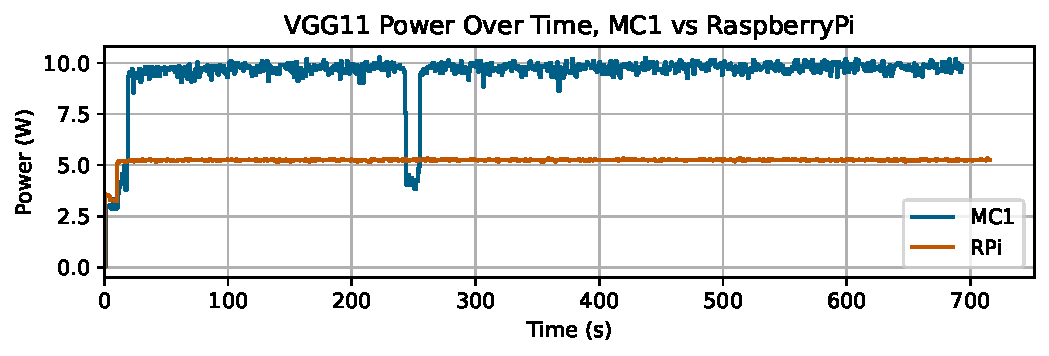
\includegraphics[width=\textwidth]{vgg11_power.pdf}
    \caption{}
    \label{fig:vgg11-power}
\end{figure}

\begin{figure}[!htb]
    \centering
    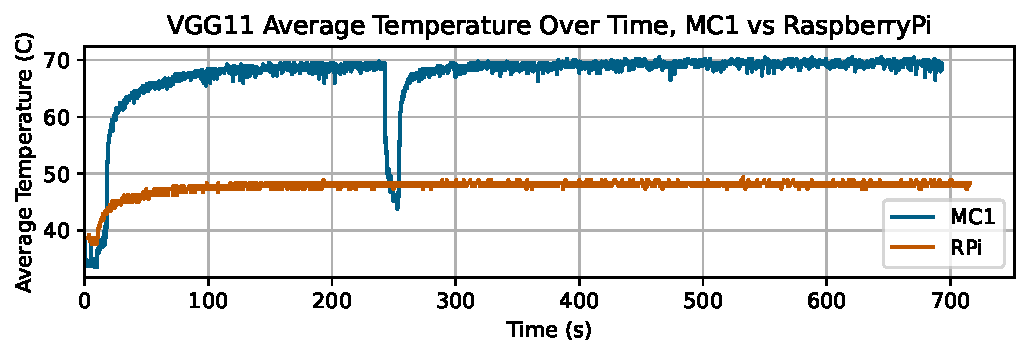
\includegraphics[width=\textwidth]{vgg11_average_temperature.pdf}
    \caption{}
    \label{fig:vgg11-avg-temp}
\end{figure}
\clearpage
\begin{figure}[!htb]
    \caption{\textit{Table 3}}
    \begin{tabularx}{\textwidth}{|c|*{2}{Y|}}
        \hline
        Model & MC1 Total Energy Consumption [J] & RPi total Energy Consumption [J] \\
        \hline
        VGG11 & 6574.78 & 3739.40 \\
        \hline
        VGG16 & 10106.79 & 6381.64 \\
        \hline
        MobileNet & 4196.58 & 1877.45 \\
        \hline
    \end{tabularx}
    \label{fig:deploy-energy}
\end{figure}

Considering only VGG11 and VGG16 (MobileNet will be discussed in the next section), the MC1 outperforms the RaspberryPi in inference time and thus would be more suitable for a low-latency use case. However, if a strict power budget is the concern, then the RaspberryPi would be more suitable, as it consumes less power and thus outputs less heat.

Note that accuracy is identical between devices (which should be the case as both devices are executing the same model). Also, memory usage is not a good metric for performance outside of correlating with power usage, as both devices performed well under their total memory budget.

\section*{Problem 3}
\subsection*{BONUS}
The MobileNet model performs the best in terms of composite performance across both platforms.
It is the most energy efficient model, is the fastest model in terms of inference, and has 
accuracy on par with the other two models.

MobileNet's key advantage is the usage of depthwise convolution, which significantly reduces the computation cost of the forward pass on convolutional layers.
Depthwise convolution works by splitting the convolution operation into two steps. First, a single filter is applied to each input channel, which is followed by a pointwise convolution to combine the output channels into one output.

This is significantly faster than convolving one learned filter with the entire input tensor. 

\section*{Contributions and Valuable Things Learned}
Both group members, Sidharth Babu and Tianda Huang, contributed an equal amount of work due to working on the entire project together.

We learned about the importance of edge-device tuned models in achieving efficiency and high performance: the reduced power, model size, and inference time of MobileNet-v1 compared to VGG11 and VGG16 is a clear demonstration.

Additionally, we observed the diminishing marginal returns of increased model complexity, seen as the very small accuracy improvement between VGG11 and VGG16 constrasting with the increase in MACs, power usage, and inference/training time that VGG16 demands.

\end{document}